\documentclass{article}
\usepackage{tikz}
\usetikzlibrary{arrows,shapes,positioning,calc}

\begin{document}

% Increase page size and diagram size
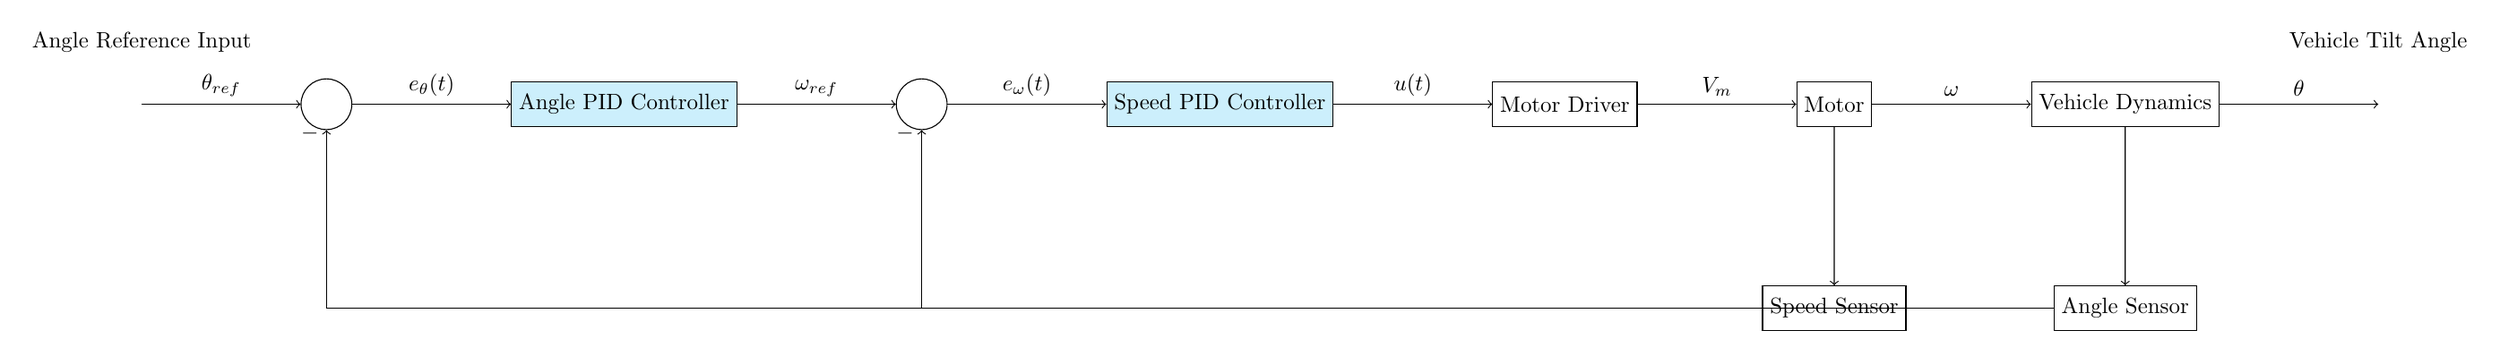
\begin{tikzpicture}[auto, 
    node distance=3cm, % Increase node distance
    scale=0.9, % Overall scaling to fit the page
    transform shape,
    block/.style={rectangle, draw, fill=white, minimum height=2em, minimum width=2.5em},
    sum/.style={circle, draw, minimum size=0.8cm},
    input/.style={coordinate},
    output/.style={coordinate}]
    
    % Outer loop nodes (Angle control)
    \node [input, name=input] (angle_input) {};
    \node [sum, right=2.5cm of angle_input] (angle_sum) {};
    \node [block, right=2.5cm of angle_sum, fill=cyan!20] (angle_controller) {Angle PID Controller};
    
    % Inner loop nodes (Speed control)
    \node [sum, right=2.5cm of angle_controller] (speed_sum) {};
    \node [block, right=2.5cm of speed_sum, fill=cyan!20] (speed_controller) {Speed PID Controller};
    \node [block, right=2.5cm of speed_controller] (driver) {Motor Driver};
    \node [block, right=2.5cm of driver] (motor) {Motor};
    
    % Vehicle dynamics
    \node [block, right=2.5cm of motor] (dynamics) {Vehicle Dynamics};
    \node [output, right=2.5cm of dynamics] (angle_output) {};
    
    % Sensors
    \node [block, below=2.5cm of dynamics] (angle_sensor) {Angle Sensor};
    \node [block, below=2.5cm of motor] (speed_sensor) {Speed Sensor};
    
    % Connections - Outer loop
    \draw [->] (angle_input) -- node {$\theta_{ref}$} (angle_sum);
    \draw [->] (angle_sum) -- node {$e_\theta(t)$} (angle_controller);
    \draw [->] (angle_controller) -- node {$\omega_{ref}$} (speed_sum);
    
    % Connections - Inner loop
    \draw [->] (speed_sum) -- node {$e_\omega(t)$} (speed_controller);
    \draw [->] (speed_controller) -- node {$u(t)$} (driver);
    \draw [->] (driver) -- node {$V_m$} (motor);
    \draw [->] (motor) -- node {$\omega$} (dynamics);
    \draw [->] (dynamics) -- node {$\theta$} (angle_output);
    
    % Feedback connections
    \draw [->] (dynamics) -- ($(dynamics)+(0,-1.25cm)$) -| (angle_sensor);
    \draw [->] (angle_sensor) -| node[pos=0.99] {$-$} (angle_sum);
    
    \draw [->] (motor) -- ($(motor)+(0,-1.25cm)$) -| (speed_sensor);
    \draw [->] (speed_sensor) -| node[pos=0.99] {$-$} (speed_sum);
    
    % Labels
    \node [above=0.7cm of angle_input] {Angle Reference Input};
    \node [above=0.7cm of angle_output] {Vehicle Tilt Angle};
    
\end{tikzpicture}

\end{document}
